\documentclass{beamer}
%\usepackage{ngerman}
\usepackage{soul}
\usepackage{mathtools}
\usepackage{amssymb,amsmath,amsfonts}
\usepackage[utf8]{inputenc}
\usepackage{graphicx}
\usepackage{float}
\usepackage[autostyle=true,german=quotes]{csquotes}
\usepackage{gensymb}
\usepackage{units}
\usepackage{fancyhdr}
\usepackage[font=small,labelfont=bf]{caption}
\usepackage[%backend=biber,
citestyle=authortitle,
sorting=nty
]{biblatex}


\addbibresource{../../lib/lib.bib}
\addbibresource{../../solensim.bib}
\graphicspath{{../../figures/}}

\setbeamertemplate{navigation symbols}{}
%\setbeamertemplate{bibliography item}{\insertbiblabel}
\setbeamertemplate{section in toc}[square]
\setbeamertemplate{subsection in toc}[square]
\setbeamertemplate{footline}[frame number]

\title{Report 15.09.20}
%\subtitle{Subtitle}
%\author{Author 1 \and Author 2}
%\date{DATE \today}

\begin{document}
%Title slide:
%\begin{frame}[plain]
%  \titlepage
%\end{frame}

%TOC slide:
%\begin{frame}
%  \frametitle{Structure}
%  \tableofcontents%[currentsection]
%\end{frame}

\begin{frame}
  \frametitle{Beam rotation}
  \framesubtitle{Qualitative observations}
  \begin{figure}
    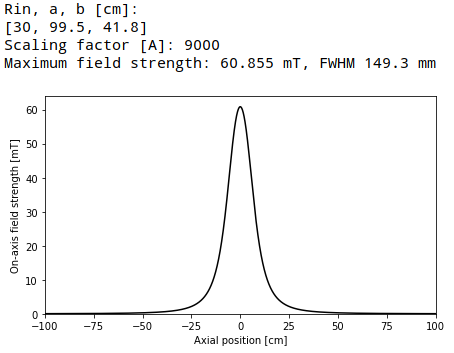
\includegraphics[width=0.7\textwidth]{field_101}
    \caption{Field profile used so far}
  \end{figure}
\end{frame}

\begin{frame}
  \frametitle{Beam rotation}
  \framesubtitle{Qualitative observations}
  \begin{figure}
    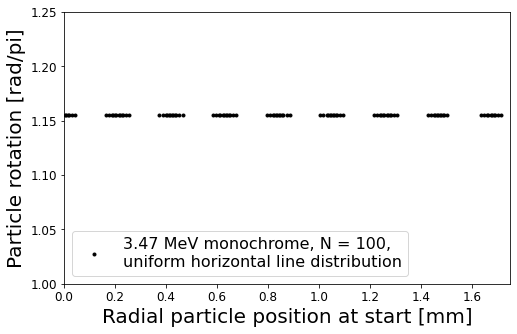
\includegraphics[width=0.7\textwidth]{rot_line_3.47_mono_100}
    \caption{Particle rotation does not seem to depend on the beam's radial distribution. \\(The particles had no starting transverse momentum)}
  \end{figure}
\end{frame}

\begin{frame}
  \frametitle{Beam rotation}
  \framesubtitle{Qualitative observations}
  \begin{figure}
    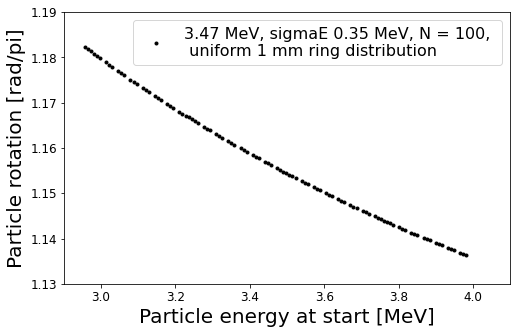
\includegraphics[width=0.7\textwidth]{rot_ring_3.47_pm10_100}
    \caption{Particle rotation exhibits slight inverse proportionality to particle energy.\\(The particles had no starting transverse momentum)}
  \end{figure}
\end{frame}

\begin{frame}
  \frametitle{Beam rotation}
  \framesubtitle{Qualitative observations}
  \begin{figure}
    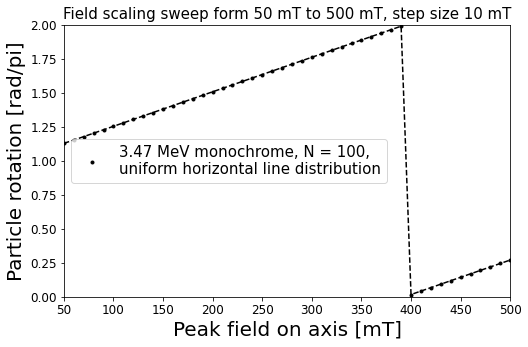
\includegraphics[width=0.7\textwidth]{line_bmax_sweep}
    \caption{Beam rotation is linearly proportional to maximum field strength.\\(The particles had no starting transverse momentum)}
  \end{figure}
\end{frame}

\begin{frame}
  \frametitle{Beam rotation}
  \framesubtitle{Qualitative observations}
  \begin{figure}
    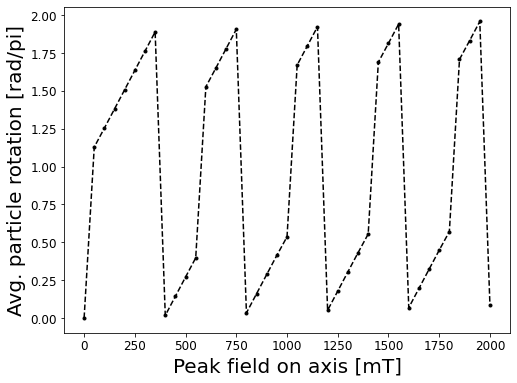
\includegraphics[width=0.7\textwidth]{wtf}
    \caption{??? No idea, why the jumps. Could be \textquotedblleft nonlinear effects\textquotedblright, could be unreasonable field strengths - for ASTRA, and in general.}
  \end{figure}
\end{frame}

%\section{Section 2}
%\begin{frame}%
  %\frametitle{Title}
  %\framesubtitle{Subtitle}
%\end{frame}

%\section{Summary}
%\begin{frame}
%  \frametitle{Summary}
%  \framesubtitle{Subtitle}
%\end{frame}

%\begin{frame}[allowframebreaks]
%  \frametitle{References}
%  \printbibliography
%\end{frame}

\end{document}
